\documentclass[11pt]{article}
\usepackage[utf8]{inputenc}
\usepackage{amsfonts,epsfig}
\usepackage[hyphens]{url}
\usepackage{hyperref}
\usepackage{breakurl}
\usepackage{comment}

% \usepackage[
% scale=.875,
% stdmathitalics=true,
% stdmathdigits=true]{lucimatx}
\linespread{1.02}

\usepackage{relsize}
\usepackage{fancyvrb}
\usepackage{amsmath, amssymb}
%%% Document layout, margins
\usepackage{geometry}
\geometry{letterpaper, textwidth=6.5in, textheight=9in, marginparsep=1em}
%%% Section headings
\usepackage{sectsty}
\usepackage{caption}
\usepackage{subcaption}
% \usepackage[export]{adjustbox}
\usepackage[normalem]{ulem}
\sectionfont{\sffamily\bfseries\upshape\large}
\subsectionfont{\sffamily\bfseries\upshape\normalsize}
\subsubsectionfont{\sffamily\mdseries\upshape\normalsize}
\makeatletter
\renewcommand\@seccntformat[1]{\csname the#1\endcsname.\quad}
\makeatother\renewcommand{\bibitem}{\vskip 2pt\par\hangindent\parindent\hskip-\parindent}

\makeatletter
\def\@maketitle{%
  \begin{center}%
  \let \footnote \thanks
    {\large \@title \par}%
    {\normalsize
      \begin{tabular}[t]{c}%
        \@author
      \end{tabular}\par}%
    {\small \@date}%
  \end{center}%
}
\makeatother


\title{\bf R-squared for Bayesian model fits\footnote{We thank Frank Harrell for helpful comments and the National Science Foundation, Office of Naval Research, Institute for Education Sciences, and Sloan Foundation for partial support of this work.}\vspace{.1in}}
\author{Andrew Gelman\footnote{Department of Statistics and Department of Political Science, Columbia University.} \and Ben Goodrich\footnote{Institute for Social and Economic Research and Policy, Columbia University.} \and Jonah Gabry$^\ddagger$ \and Imad Ali\footnote{Department of Statistics, Columbia University.}\vspace{.1in}}
\date{25 July 2017\vspace{-.1in}}
\begin{document}\sloppy
\maketitle
\thispagestyle{empty}

\begin{abstract}
The usual definition of $R^2$ (variance of the predicted values divided by the
variance of the data) has a problem for Bayesian fits, as the numerator can be
larger than the denominator.  We propose an alternative definition similar to 
one that has appeared in the survival analysis literature:  the variance of the 
predicted values divided by the variance of predicted values plus variance of 
the errors. Our plan is for this to be printed automatically for linear and 
generalized linear regression models fit using {\tt rstanarm}, our R package 
that fits Bayesian regression models using Stan.
\end{abstract}

\section{The problem}

Consider a regression model of outcomes $y$ and predictors $X$ with predicted
values $\mbox{E}(y|X,\theta)$, fit to data $(X,y)_i, i=1,\ldots,n$.  Ordinary
least squares regression yields an estimated parameter vector $\hat{\theta}$
with predicted values $\hat{y}_i=\mbox{E}(y|X_i,\hat{\theta})$ and residual
variance $V_{i=1}^n \hat{y}_i$, where we are using the notation,
%
$$
V_{i=1}^nz_i = \frac{1}{n-1}\sum_{i=1}^n(z_i-\bar{z})^2, \mbox{ for any vector }z.
$$
%
The proportion of variance explained,
%
\begin{equation}\label{rsq1}
\mbox{classical } R^2=\frac{V_{i=1}^n\hat{y}_i}{V_{i=1}^n y_i},
\end{equation}
%
is a commonly used measure of model fit, and there is a long literature on
interpreting it, adjusting it for degrees of freedom used in fitting the model,
and generalizing it to other settings such as hierarchical models; see Xu (2003)
and Gelman and Pardoe (2006).

Here we consider how to extend the concept of $R^2$ to apply to Bayesian model
fitting.  Our motivation is the package {\tt rstanarm} (Gabry and Goodrich,
2017), which contains a set of wrapper functions that allows the user to express
regression models using traditional R syntax
(for example, $\mathtt{y \sim x1 + x2 + x3}$)
and then fit these models using Bayesian inference, allowing the incorporation
of prior information in the input stage and yielding posterior simulations and
predictions in the output.  After fitting a model using the \verb#stan_glm()#
or \verb#stan_glmer()# function, we would like to display an estimate of $R^2$ 
along with the estimated coefficients and standard errors.

\section{Defining $R^2$ based on the variance of estimated prediction errors}

Our first thought for Bayesian $R^2$ is to simply use the posterior mean
estimate of $\theta$ to create Bayesian predictions $\hat{y}_i$ and then plug
these into the classical formula \eqref{rsq1}.  This has two problems:  first,
it is dismisses uncertainty to use a point estimate in Bayesian computation;
and, second, the ratio as thus defined can be greater than 1.  When
$\hat{\theta}$ is estimated using ordinary least squares, and assuming the
regression model includes a constant term, the numerator of \eqref{rsq1} is less
than or equal to the denominator by definition; more generally, though, there is
no requirement that this be the case, and it would be awkward to say that a
fitted model explains more than 100\% of the variance.

\begin{figure}
\centerline{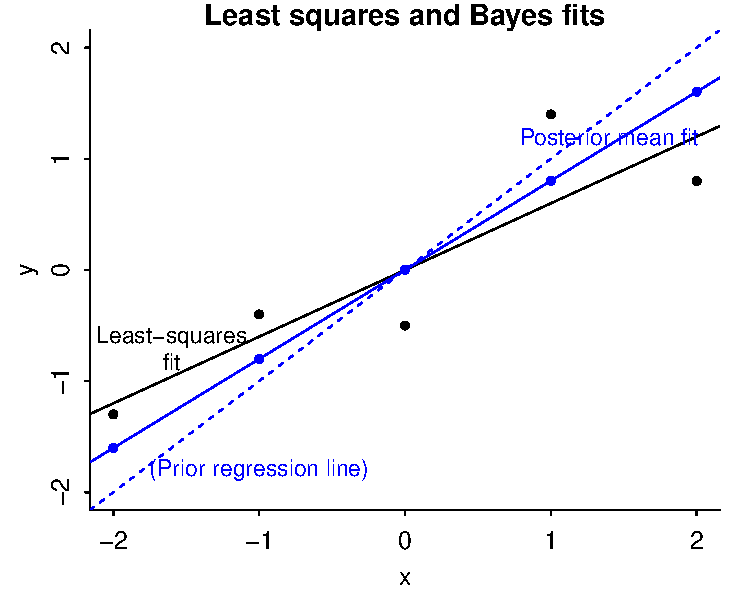
\includegraphics[width=.5\textwidth]{fig/rsquared1a.pdf}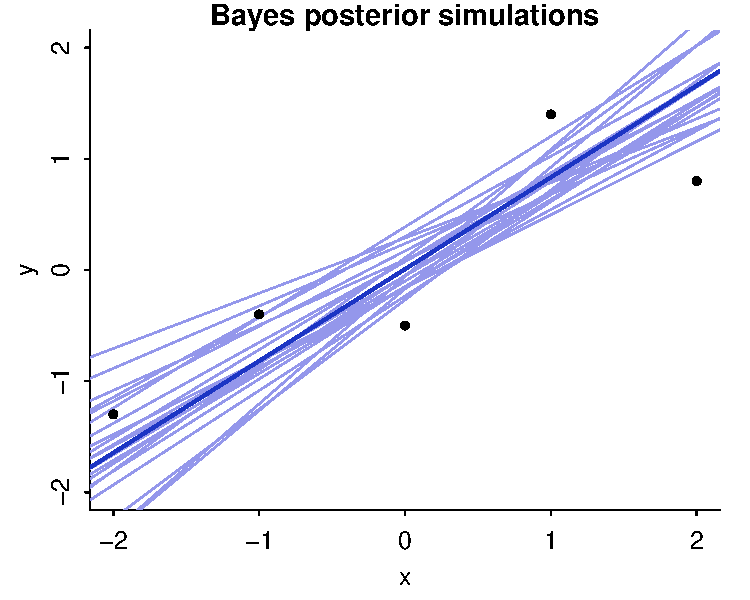
\includegraphics[width=.5\textwidth]{fig/rsquared1b.pdf}}
\vspace{-.1in}
\caption{\em Simple example showing the challenge of defining $R^2$ for a fitted
Bayesian model.  {\em Left plot:}  data, least-squares regression line, and
fitted Bayes line, which is a compromise between the prior and the least-squares
fit.  The standard deviation of the fitted values from the Bayes model (the blue
dots on the line) is greater than the standard deviation of the data, so the
usual definition of $R^2$ will not work.  {\em Right plot:}  posterior mean
fitted regression line along with 20 draws of the line from the posterior
distribution.  To define a Bayesian $R^2$ we compute equation 
\eqref{rsq3} for each posterior simulation draw and then take the median.}
\label{rsquared1}
\end{figure}

To see an example where the simple $R^2$ would be inappropriate, consider a model
$y = \alpha + \beta x+\mbox{error}$
with a strong prior on $(\alpha,\beta)$ and only a few data points.
Figure~\ref{rsquared1}a shows data and the least-squares regression line (with
$R^2$ of 0.77).  We then do a Bayes fit with informative priors
$\alpha \sim \mbox{N}(0,0.2^2)$ and $\beta \sim \mbox{N}(1,0.2^2)$.  The
standard deviation of the fitted values from the Bayes model is 1.3, while the
standard deviation of the data is only 1.08, so the square of this
ratio---$R^2$ as defined in \eqref{rsq1}---is greater than 1.
Figure~\ref{rsquared1}b shows the posterior mean fitted regression line along
with 20 draws of the line $y = \alpha + \beta x$ from the fitted posterior
distribution of $(\alpha,\beta)$.\footnote{Code for this example is available at \url{https://github.com/jgabry/bayes_R2}.}

Instead of working with \eqref{rsq1} directly, we generalize a different formula
for explained variance:
%
\begin{equation}\label{rsq2}
\mbox{alternative } R^2 = \frac{V_{i=1}^n\hat{y}_i}{V_{i=1}^n \hat{y}_i  + V_{i=1}^n r_i},
\end{equation}
%
where $r_i = y_i -\hat{y}_i$ are the residuals of the fitted model.
The advantage of \eqref{rsq2} is that it is always between $0$ and $1$ by
construction, no matter what procedure is used to construct the estimate
$\hat{y}$.

Versions of expression \eqref{rsq2} have appeared in the survival analysis
literature (Kent and O'Quigley, 1988, Choodari-Oskoo, Royston, and Parmar,
2010), where it makes sense to use expected rather than observed data variance
in the denominator.  Our motivation is slightly different but the same
mathematical principles apply.

In Bayesian inference we do not have a point estimate $\hat{\theta}$ but rather
a set of posterior simulation draws, $\theta^s, s=1,\ldots,S$.
For each $\theta^s$, we can compute the vector of predicted values
$\hat{y}_i^s = \mbox{E}(y | X_i,\theta^s)$, the vector of errors
$e_i^s = y_i^s - \hat{y}_i^s$, and thus the proportion of variance explained,
%
\begin{equation}\label{rsq3}
\mbox{Bayesian } R^2_s=\frac{V_{i=1}^n\hat{y}_i^s}{V_{i=1}^n \hat{y}_i^s  + V_{i=1}^n e_i^s}.
\end{equation}
%
We can then summarize this by its posterior median, for example. It would also
be possible to obtain an estimate of the posterior uncertainty in $R^2$,
although it is not clear that this would be of much interest.

For a linear regression model we can compute the Bayesian $R^2$ defined in
\eqref{rsq3} using the \verb#posterior_linpred# function in the {\tt rstanarm}
package (Gabry and Goodrich, 2017) and a few additional lines of code:
%
\vspace{-\baselineskip}
\begin{quotation}
\noindent
\begin{small}
\begin{verbatim}
bayes_R2 <- function(fit) {
  y <- get_y(fit)
  ypred <- posterior_linpred(fit)
  e <- -1 * sweep(ypred, 2, y)
  var_ypred <- apply(ypred, 1, var)
  var_e <- apply(e, 1, var)
  var_ypred / (var_ypred + var_e)
}
## Example
M1 <- stan_glm(y ~ x)
print(median(bayes_R2(M1)))
\end{verbatim}
\end{small}
\end{quotation}
%
For the example in Figure~\ref{rsquared1}, the median $R^2$ from
equation \eqref{rsq3}, as calculated by the above code, is 0.80.  In comparison,
if we were to replace the denominator of \eqref{rsq3} by $V_{i=1}^n y_i$, we
would get a median $R^2$ of 1.44.  Also, in case it might be of interest, we
report the posterior mean and standard deviation of $R^2$ in this example:
they are 0.79 and 0.03.

\section{Models with group-specific terms}
The {\tt rstanarm} package also provides the \verb#stan_glmer# function for 
fitting models with group-specific coefficients that have unknown covariance matrices.
The linear predictor for these models is often written as $X \beta + Zb$. 
In the classical formulation $Zb$ can be considered as part of the model's error term
rather than the conditional mean of the outcome, but from a Bayesian perspective we 
condition on $Z$ when fitting the model and it makes sense by default to include the $Zb$ 
term when computing $\hat{y}$. However, the \verb#bayes_R2# function in {\tt rstanarm} will 
provide an {\tt re.form} argument that allows the user to override this default and specify which, 
if any, of the group-level terms should factor into the computation of $\hat{y}$ and thus $R^2$. 

\section{Discussion}
$R^2$ has well-known problems as a measure of model fit, but it can be a handy
quick summary for linear regressions and generalized linear models (see, for
example, Hu, Palta, and Shao, 2006) and we would like to produce it by default
when fitting Bayesian regressions.  Our preferred solution is to use the
posterior median of the ratio \eqref{rsq3}:  predicted variance divided by
predicted variance plus error variance.

A new issue then arises, though, when fitting a set of a models to a single
dataset.  Now that the denominator of $R^2$ is no longer fixed, we can no longer
interpret an increase in $R^2$ as a improved fit to a fixed target.  We think
this particular loss of interpretation is necessary:  from a Bayesian
perspective, a concept such as ``explained variance'' can ultimately only be
interpreted in the context of a model.  The denominator of \eqref{rsq3} can be
interpreted as an estimate of the expected variance of predicted future data
from the model under the assumption that the predictors $X$ are held fixed;
alternatively the predictors can be taken as random, as suggested by Helland
(1987) and Tjur (2009).  In either case, we can consider our Bayesian $R^2$ as a
data-based estimate of the proportion of variance explained for new data. If the
goal is to see continual progress of the fit to existing data, one can simply
track the decline in the estimated error variance, $V_{i=1}^n e_i^s$.

Moving forward, we plan to implement our Bayesian $R^2$ by default in
{\tt rstanarm}, not just for linear regression but also for generalized linear
models; see the appendix for a generalized version of the
\verb#bayes_R2# function. The concept of ``explained variance'' makes most
sense for linear models with equal variance, but given that we can essentially
compute $R^2$ for free, we might as well do so.  An alternative is to summarize
residual error on the log-probability scale, in which case we recommend using
approximate leave-one-out cross-validation (Vehtari, Gelman, and Gabry, 2017),
which can be done using the {\tt loo()} function within {\tt rstanarm}.   If
desired, changes in expected log-probability scores can be converted back to an
$R^2$ scale as discussed by Nagelkerke (1991).

One issue that arises when using $R^2$ to evaluate and compare models is
overfitting.  As with other measures of predictive model fit, overfitting should
be less of an issue with Bayesian inference because averaging over the posterior
distribution is more conservative than taking a least-squares or maximum
likelihood fit, but predictive accuracy for new data will still on average be
lower, in expectation, than for the data used to fit the model (Gelman, Hwang,
and Vehtari, 2014).   We will include a {\tt newdata} argument in the \verb#bayes_R2# 
function  that can be used in the case that new or held-out data are actually 
available, but otherwise to correct for that bias one might want to replace
$V_{i=1}^n e_i^s$ in the denominator of \eqref{rsq3} by its expectation for new
data, or more generally one could construct an overfitting-corrected $R^2$ in
the same way that is done for log-score measures via cross-validation. 
In the present paper we are trying to stay close to the sprit of the original $R^2$ in
quantifying the model's fit to the data at hand.


\section*{References}

\noindent

\bibitem Choodari-Oskoo, B., Royston, P., and Parmar, M. K. B. (2010).  A simulation study of predictive ability measures in a survival model I: Explained variation measures.  {\em Statistics in Medicine} {\bf 31}, 2627--2643.

\bibitem Gabry, J., and Goodrich, B. (2017).  rstanarm:  Bayesian applied regression modeling via Stan.  \url{https://cran.r-project.org/web/packages/rstanarm/index.html}

\bibitem Gelman, A., Hwang, J., and Vehtari, A. (2014).  Understanding predictive information criteria for Bayesian models. {\em Statistics and Computing} {\bf 24}, 997--1016.

\bibitem Gelman, A., and Pardoe, I. (2006).  Bayesian measures of explained variance and pooling in multilevel (hierarchical) models. {\em Technometrics} {\bf 48}, 241--251.

\bibitem Helland, I. S. (1987).  On the interpretation and use of $R^2$ in regression analysis.  {\em Biometrics} {\bf 43}, 61--69.

\bibitem Hu, B., Palta, M., and Shao, J. (2006).  Properties of $R^2$ statistics for logistic regression.  {\em Statistics in Medicine} {\bf 25}, 1383--1395.

\bibitem Kent, J. T., and O'Quigley, J. (1988). Measures of dependence for censored survival data. {\em Biometrika} {\bf 75}, 525--534.

\bibitem Nagelkerke, N. J. D. (1991).  A note on a general definition of the coefficient of determination. {\em Biometrika} {\bf 78}, 691--692.

\bibitem Tjur, T. (2009).  Coefficient of determination in logistic regression models---A new proposal:  The coefficient of discrimination.  {\em American Statistician} {\bf 63}, 366--372.

\bibitem Vehtari, A., Gelman, A, and Gabry, J. (2017).  Practical Bayesian model evaluation using leave-one-out cross-validation and WAIC. {\em Statistics and Computing} {\bf 27}, 1413--1432.

\bibitem Xu, R. (2003).  Measuring explained variation in linear mixed-effects models.  {\em Statistics in Medicine} {\bf 22}, 3527--3541.

\pagebreak

\section*{Appendix}

This modified version of the \verb#bayes_R2# function works with
Bayesian linear and generalized linear models fit using the 
\verb#stan_glm# function in the {\tt rstanarm} package. The only 
differences compared to the function presented in the body of the paper are 
the requirement of specifying \verb#transform=TRUE# in the call to 
\verb#posterior_linpred# (to apply the inverse-link function to the linear 
predictor) and a few lines to account for the binomial models that
have a number of trials greater than 1. 
%
\vspace{-\baselineskip}
\begin{quotation}
\noindent
\begin{small}
\begin{verbatim}
# Compute Bayesian R-squared for linear and
# generalized linear models.
#
# @param fit A fitted model object returned by stan_glm.
# @return A vector of R-squared values with length equal to
#      the number of posterior draws.
#
bayes_R2 <- function(fit) {
  y <- get_y(fit)
  ypred <- posterior_linpred(fit, transform = TRUE)
  if (family(fit)$family == "binomial" && NCOL(y) == 2) {
    trials <- rowSums(y)
    y <- y[, 1]
    ypred <- ypred %*% diag(trials)
  }
  e <- -1 * sweep(ypred, 2, y)
  var_ypred <- apply(ypred, 1, var)
  var_e <- apply(e, 1, var)
  var_ypred / (var_ypred + var_e)
}
\end{verbatim}
\end{small}
\end{quotation}

\noindent The code for the \verb#bayes_R2# function included in {\tt rstanarm} will be 
more complicated than the function presented here in order to accommodate models fit 
using \verb#stan_glmer# and various special cases.

\end{document}
